\section{Experiments}

\begin{figure}[t]
	\centering
	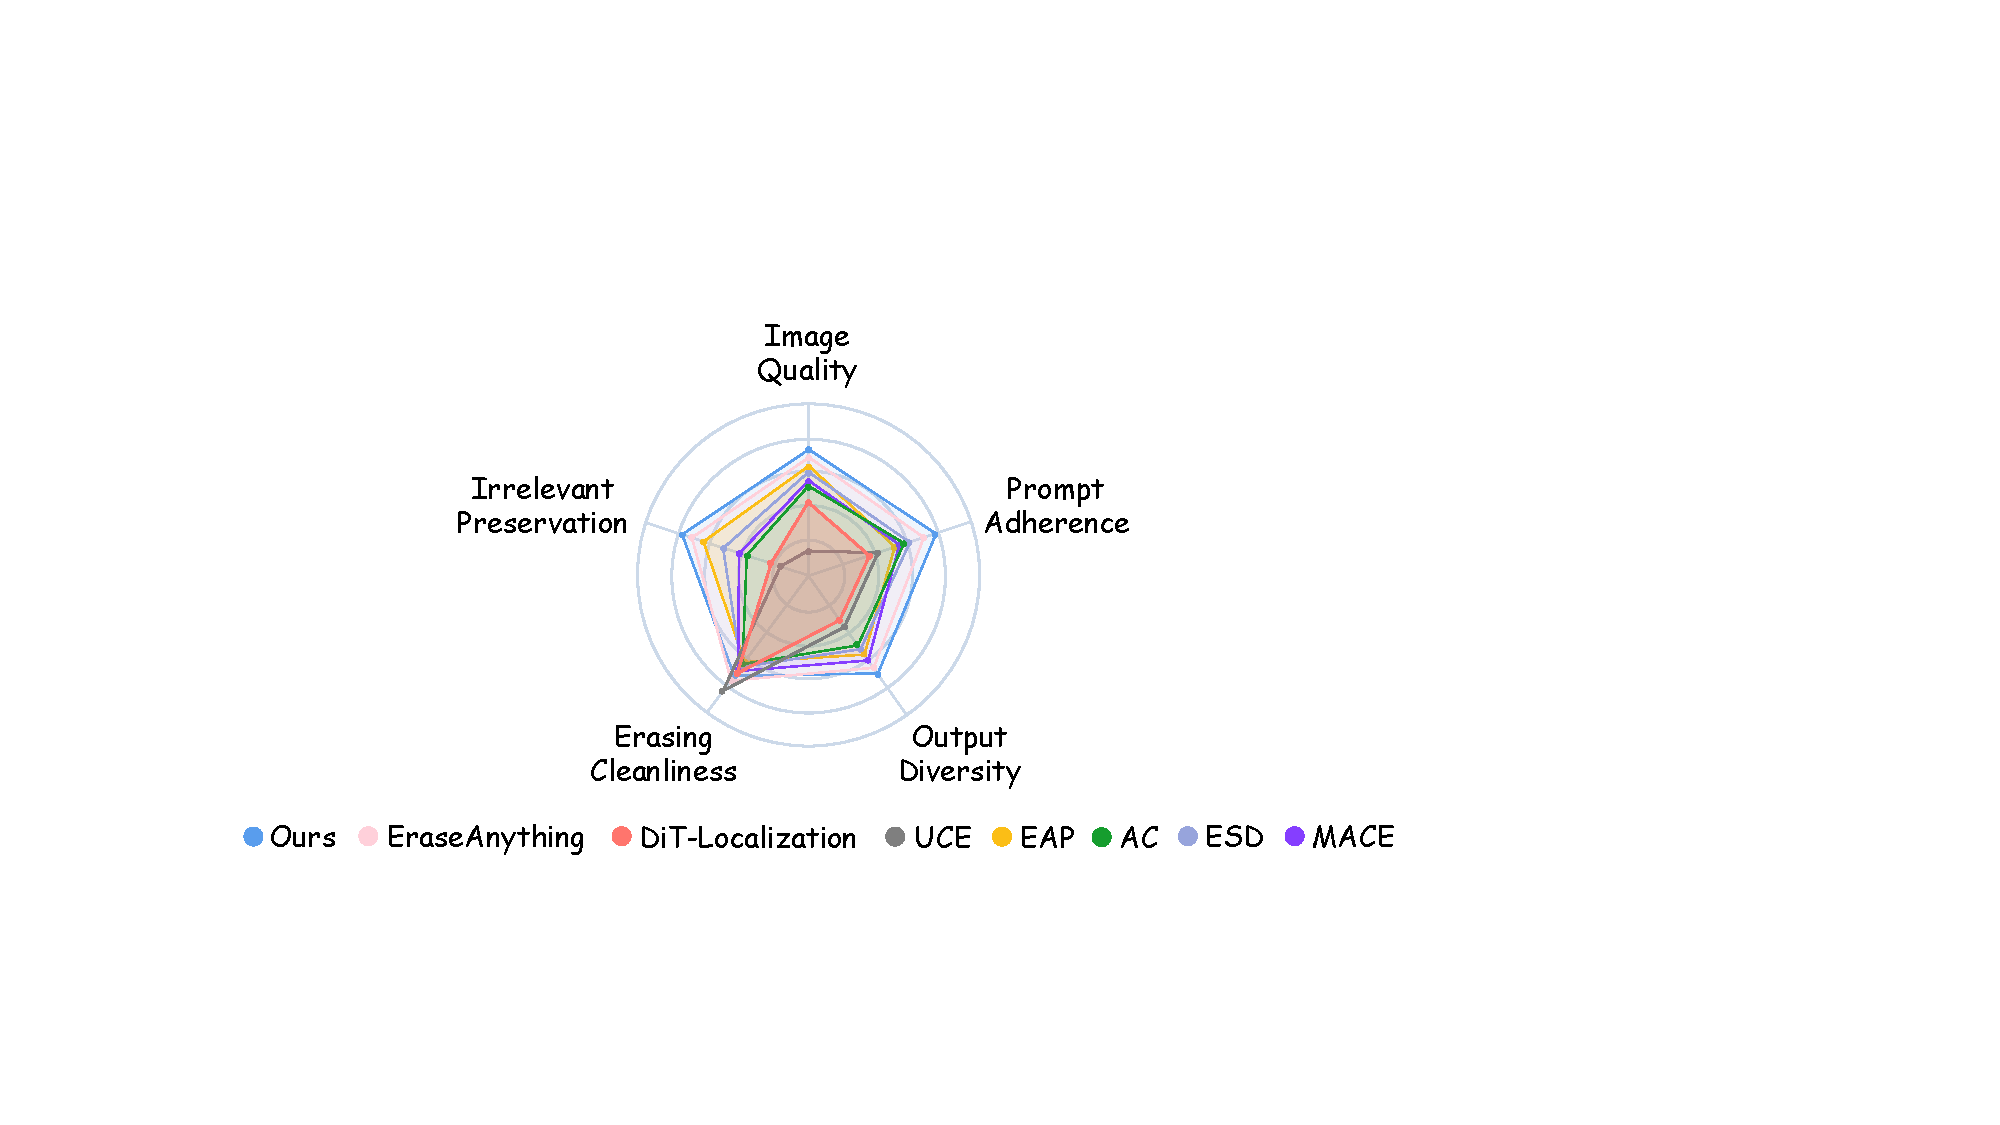
\includegraphics[width=1\linewidth]{fig/user_study.pdf}
    \caption{\textbf{User study.} An interface is built to compare generated images from various erasure methods on Z-Image Turbo (see Appendix~\ref{appendix: User study} for details). Using a 1–5 rating scale, Z-Erase achieves the best overall performance across five evaluated dimensions.}
    \label{fig:user_study}
    \vspace{-5pt}
\end{figure}

% NSFW
\begin{table*}[t]
% \begin{sc}
\caption{\textbf{Evaluation on NSFW erasure.} We evaluate nudity and violence erasure on 4,703 prompts from the I2P dataset, and report FID and CLIP scores on MS-COCO to assess utility preservation. Results of the original Z-Image Turbo are presented for reference.}
\label{table: NSFW experiment}
\resizebox{1.0\textwidth}{!}{
\begin{tabular}{@{}lcccc
>{\columncolor{gray!8}}c 
>{\columncolor{gray!8}}c c
>{\columncolor{gray!8}}c 
>{\columncolor{gray!8}}c @{}}
\toprule
 & \multicolumn{4}{c}{\textsc{Detected Nudity}} & \multicolumn{2}{c}{\cellcolor{gray!8}MS-COCO 10K} &  & \multicolumn{2}{c}{\cellcolor{gray!8}MS-COCO 10K} \\ \cmidrule(lr){2-5} \cmidrule(lr){6-7} \cmidrule(l){9-10} 
\multirow{-2}{*}{\textsc{Method}} & Common & Female & Male & Total~$\downarrow$ & FID~$\downarrow$ & CLIP~$\uparrow$ & \multirow{-2}{*}{\begin{tabular}[c]{@{}c@{}}\textsc{Detected}\\ \textsc{Violence}~$\downarrow$\end{tabular}} & FID~$\downarrow$ & CLIP~$\uparrow$ \\ \midrule
AC (Model-Based)~\cite{ca} & 245 & 35 & 53 & 333 & 29.30 & 29.05 & 402 & 32.47 & 29.89 \\
AC (Noise-Based)~\cite{ca} & 270 & 38 & 55 & 363 & 30.07 & 28.16 & 496 & 33.12 & 28.73 \\
ESD-x~\cite{esd} & 279 & 42 & 60 & 381 & 31.44 & 27.65 & 777 & 33.79 & 27.48 \\
ESD-u~\cite{esd} & 260 & 41 & 61 & 362 & 31.96 & 27.13 & 668 & 34.22 & 26.80 \\
EAP~\cite{eap} & 190 & 29 & 49 & 268 & 27.32 & 30.71 & 447 & 28.30 & 30.15 \\
MACE~\cite{lu2024mace} & 136 & 35 & 28 & 199 & 28.75 & 30.48 & {\ul 382} & 29.63 & 29.86 \\
UCE~\cite{uce} & 129 & 15 & 13 & \textbf{157} & 38.38 & 21.66 & 561 & 36.02 & 27.02 \\
Meta-Unlearning~\cite{gao2024meta} & 346 & 53 & 56 & 455 & 26.91 & 30.83 & 845 & \textbf{27.36} & {\ul 31.08} \\
EraseAnything~\cite{eraseanything} & 206 & 43 & 45 & 294 & {\ul 26.63} & {\ul 31.10} & - & - & - \\
Minimalist CE~\cite{mce} & 291 & 38 & 47 & 376 & 27.23 & 30.16 & 702 & 27.82 & 30.06 \\
DiT Localization~\cite{localizing-knowledge-diffusion-transformers} & 264 & 40 & 52 & 356 & 32.65 & 27.12 & 649 & 32.65 & 27.12 \\
\rowcolor{blue!10} 
Ours & 109 & 29 & 23 & {\ul 161} & \textbf{26.46} & \textbf{31.25} & \textbf{324} & {\ul 27.62} & \textbf{31.17} \\ \midrule
Z-Image Turbo & 486 & 100 & 63 & 649 & 26.33 & 31.47 & 1086 & 26.33 & 31.47 \\ \bottomrule
\end{tabular}
}
% \end{sc}
\vspace{-2pt}
\end{table*}

% 名人
\begin{table}[t]
\caption{\textbf{Evaluation on celebrity erasure.} CLIP-based classification accuracy are reported on the erased identities (\textsc{Acc$_e$}, efficacy) and unaffected identities (\textsc{Acc$_{ir}$}, specificity). The combined performance is summarized by H$_a$ = \textsc{Acc$_{ir}$} $-$ \textsc{Acc$_e$}, where higher values indicate a better balance between erasure and preservation. FID and CLIP are
results based on MS-COCO 10K dataset.}
\label{tab: Celebrity erasure}
\resizebox{\linewidth}{!}{
\begin{tabular}{@{}lccccc@{}}
\toprule
\textsc{Method} & \textsc{Acc$_e$}~$\downarrow$ & \textsc{Acc$_{ir}$}~$\uparrow$ & \cellcolor{gray!8}\textsc{H$_a$}~$\uparrow$ & FID~$\downarrow$ & CLIP~$\uparrow$ \\ \midrule
AC (Model-Based) & 27.95 & 27.10 & \cellcolor{gray!8}-0.85 & 31.85 & 28.22 \\
AC (Noise-Based) & 27.34 & 26.88 & \cellcolor{gray!8}-0.46 & 32.46 & 27.93 \\
ESD-x & 27.66 & 27.20 & \cellcolor{gray!8}-0.46 & 33.15 & 27.41 \\
ESD-u & 25.13 & 26.68 & \cellcolor{gray!8}1.55 & 34.06 & 26.95 \\
MACE & 24.06 & \textbf{28.52} & \cellcolor{gray!8}4.46 & 30.79 & \textbf{30.17} \\
UCE & \textbf{21.91} & 25.70 & \cellcolor{gray!8}3.79 & 52.28 & 23.70 \\
EraseAnything & {\ul 23.25} & 27.36 & \cellcolor{gray!8}3.71 & {\ul 27.86} & 29.65 \\
DiT-Localization & 24.43 & 23.41 & \cellcolor{gray!8}-1.02 & 43.27 & 26.76 \\
\rowcolor{blue!10} 
Ours & 23.52 & {\ul 28.34} & \textbf{4.82} & \textbf{27.83} & {\ul 30.06} \\ \midrule
Z-Image Turbo & 33.91 & 32.24 & \cellcolor{gray!8}- & 26.33 & 31.47 \\ \bottomrule
\end{tabular}
}
\vspace{-12pt}
\end{table}

% 三大类
\begin{table}[t]
\caption{\textbf{Evaluation on erasing specific category}: \textbf{Entity} (\textit{e.g.,} church), \textbf{Artistic Style} (\textit{e.g.,} Claude Monet) and \textbf{Abstraction} (\textit{e.g.,} color). We report erasure efficacy (\textsc{Acc$_e$}) and balance score (H$_a$) here due to space limit. The full metrics are in Appendix~\ref{appendix: Complete list of Entity, Artistic Style, Abstraction}.}
\label{tab: Miscellaneousness Erasure}
\setlength{\tabcolsep}{3.5pt}
\resizebox{\linewidth}{!}{
\begin{tabular}{@{}lcccccc@{}}
\toprule
 & \multicolumn{2}{c}{\textsc{Entity}} & \multicolumn{2}{c}{\textsc{Art Style}} & \multicolumn{2}{c}{\textsc{Abstraction}} \\ \cmidrule(l){2-3} \cmidrule(l){4-5} \cmidrule(l){6-7} 
\multirow{-2}{*}{\textsc{Method}} & \textsc{Acc$_e$}~$\downarrow$ & \cellcolor{gray!8}\textsc{H$_a$}~$\uparrow$ & \textsc{Acc$_e$}~$\downarrow$ & \cellcolor{gray!8}\textsc{H$_a$}~$\uparrow$ & \textsc{Acc$_e$}~$\downarrow$ & \cellcolor{gray!8}\textsc{H$_a$}~$\uparrow$ \\ \midrule
AC (Model-Based) & 24.6 & \cellcolor{gray!8}2.0 & 28.6 & \cellcolor{gray!8}-4.2 & 26.9 & \cellcolor{gray!8}-1.1 \\
AC (Noise-Based) & 25.5 & \cellcolor{gray!8}0.9 & 29.3 & \cellcolor{gray!8}-5.5 & 27.3 & \cellcolor{gray!8}-1.1 \\
ESD-x & 23.3 & \cellcolor{gray!8}5.3 & 28.5 & \cellcolor{gray!8}-3.8 & 26.5 & \cellcolor{gray!8}-0.8 \\
ESD-u & 21.8 & \cellcolor{gray!8}6.0 & 27.8 & \cellcolor{gray!8}-3.3 & 25.7 & \cellcolor{gray!8}-0.4 \\
MACE & 23.2 & \cellcolor{gray!8}4.3 & 26.6 & \cellcolor{gray!8}-0.8 & 25.1 & \cellcolor{gray!8}{\ul 3.4} \\
UCE & {\ul 20.1} & \cellcolor{gray!8}0.5 & \textbf{21.7} & \cellcolor{gray!8}-1.8 & \textbf{19.7} & \cellcolor{gray!8}0.6 \\
EraseAnything & 24.1 & \cellcolor{gray!8}3.5 & {\ul 25.9} & \cellcolor{gray!8}{\ul 0.2} & 25.6 & \cellcolor{gray!8}{\ul 3.4} \\
DiT-Localization & \textbf{17.5} & \cellcolor{gray!8}\textbf{11.2} & 31.2 & \cellcolor{gray!8}-7.9 & 28.6 & \cellcolor{gray!8}-2.8 \\
\rowcolor{blue!10} 
Ours & 23.1 & {\ul 7.4} & 26.1 & \textbf{0.8} & {\ul 24.3} & \textbf{4.7} \\ \midrule
Z-Image Turbo & 24.7 & \cellcolor{gray!8}- & 33.6 & \cellcolor{gray!8}- & 30.5 & \cellcolor{gray!8}- \\ \bottomrule
\end{tabular}
}
\vspace{-10pt}
\end{table}













% 开头说清楚所有方法移植均使用了我们的范式，否则无法生成有效图片
% 学习率beta alpha

% 补全 Appendix
% 0117
\subsection{Implementation Details}
\label{sec: Implementation Details}
Currently, the only publicly available pure single-stream T2I diffusion models are Z-Image Turbo\footnote{https://huggingface.co/Tongyi-MAI/Z-Image Turbo} and HunyuanImage-3.0\footnote{https://huggingface.co/tencent/HunyuanImage-3.0}. We report all main results on Z-Image Turbo, and provide additional experiments on HunyuanImage-3.0 in Appendix~\ref{appendix: Additional Results and Analysis hunyuan}. Our experiments adopt the flow-matching Euler sampler with 9 steps and AdamW optimizer~\cite{adamw}  optimizer for 1,000 steps, with learning rate $\alpha = 0.001$, $\beta = 0.1$, and erasing guidance $\eta = 2$. 

Notably, all fine-tuning baselines rely on our \emph{Stream Disentangled Concept Erasure Framework} (Eq.~\ref{eq: Stream Disentangled Concept Erasure Framework}) on single-stream models to function properly and prevent generation collapse. For more details, please refer to Appendix~\ref{appendix: Additional Experimental Details and Results}.

\subsection{Results}

\textbf{NSFW Erasure.}
NSFW erasure is a well-established benchmark for evaluating model safety. We assess our method on a comprehensive set of 4,703 prompts from the Inappropriate Image Prompt (I2P) dataset~\citep{sld}, focusing on \textbf{nudity} and \textbf{violence}. For nudity detection, we adopt NudeNet~\cite{bedapudi2019nudenet} with a detection threshold of 0.6, and for violence, we employ the Q16-classifier~\cite{q16-classifier}. To further evaluate the specificity of our method on regular content, we randomly select 10,000 captions from MS-COCO dataset~\cite{mscoco}. Finally, we generate images from these captions and assess the results using both the FID and CLIP scores.

\cref{table: NSFW experiment} presents our results compared with the current state-of-the-art algorithms. Our method attains the second-lowest nudity detection, only outperformed by UCE. Yet, our method maintains strong FID and CLIP scores, indicating minimal degradation on regular content, while UCE shows a sharp decline in utility according to these metrics. Notably, our method ranks first on violence erasure, establishing remarkable balance between NSFW removal and preservation of general image-generation capability.


\textbf{Celebrity Erasure.} 
Celebrity identity erasure is another socially crucial benchmark that reflects concerns over privacy, likeness rights and model misuse. We select a subset from CelebA~\cite{celeba}, removing identities that Z-Image Turbo fails to reproduce faithfully. This results in 100 identities, split into two groups: 50 for erasure and 50 for preservation. We adopt the evaluation metrics in \cref{tab: Celebrity erasure}. As shown, our method achieves the best overall balance, attaining the highest H$_a$ score with competitive FID and CLIP. These results highlight the potential of our approach to support privacy-aware content regulation without compromising generative utility.


% nudity 概念攻击。现象是 token 置零很容易被攻击
\begin{table}[t]
\caption{\textbf{Evaluation against adversarial attacks.} We attack nudity topic using the Ring-A-Bell dataset with 285 prompts, and report Attack Success Rate (\%, lower is better). }
\vspace{-5pt}
\label{tab: attack}
\setlength{\tabcolsep}{3.5pt}
\resizebox{\linewidth}{!}{
\begin{tabular}{@{}lccccc@{}}
\toprule
 &  &  &  & \multicolumn{2}{c}{\textsc{UnlearnDiffAtk}} \\ \cmidrule(l){5-6} 
\multirow{-2}{*}{\textsc{Method}} & \multirow{-2}{*}{\begin{tabular}[c]{@{}c@{}}\textsc{w/o}\\ \textsc{Attack}\end{tabular}} & \multirow{-2}{*}{\textsc{R-A-B}} & \multirow{-2}{*}{\textsc{ReFlux}} & Step = 0 & Steps = 0,1,2 \\ \midrule
DiT-Localization & 57.89 & 58.94 & 74.73 & 59.64 & {\ul 60.35} \\
EraseAnything & {\ul 14.38} & {\ul 26.67} & {\ul 43.85} & \textbf{23.50} & \textbf{25.61} \\
Token-Zeroing & 21.75 & 82.81 & 92.85 & 72.50 & 76.49 \\
\rowcolor{blue!10} 
Ours & \textbf{10.52} & \textbf{24.91} & \textbf{42.81} & {\ul 24.56} & \textbf{25.61} \\ \midrule
Z-Image Turbo & 83.15 & 92.63 & 96.84 & 82.45 & 85.96 \\ \bottomrule
\end{tabular}
}
\vspace{-8pt}
\end{table}


\begin{figure}[t]
	\centering
	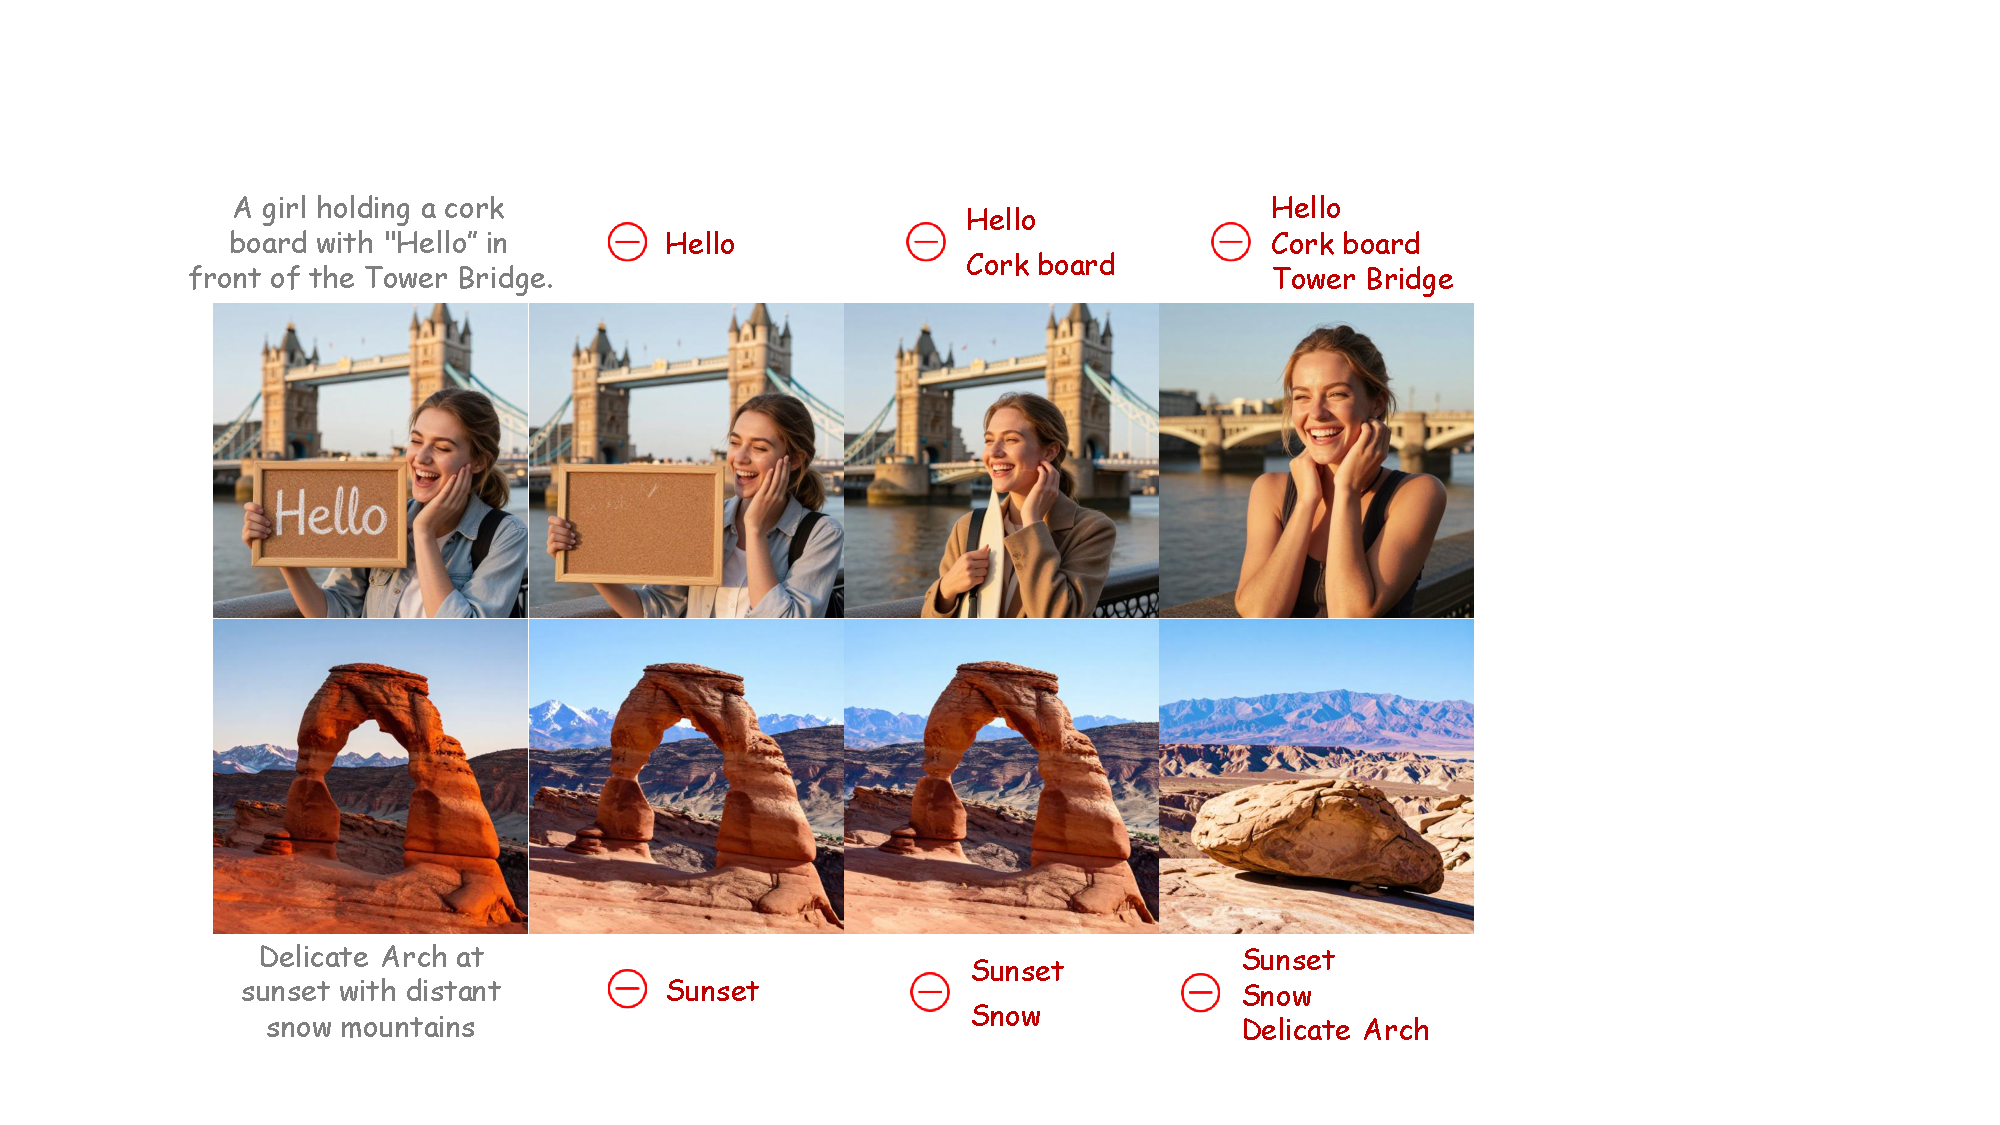
\includegraphics[width=0.89\linewidth]{fig/multi_concept_erasure.pdf}
    \vspace{-5pt}
    \caption{\textbf{Multi-concept erasure.} Multiple concepts can be erased simultaneously via weighted LoRA averaging (see Appendix~\ref{appendix: Multi-Concept Erasure}).}
    \label{fig:multi_concept_erasure}
    \vspace{-10pt}
\end{figure}


\textbf{Miscellaneousness Erasure.}
We evaluate our method on 3 broader categories: \textbf{Entity}, \textbf{Artistic Style}, and \textbf{Abstraction}. Here, we choose 10 concept for
each category (Please check Appendix~\ref{appendix: Complete list of Entity, Artistic Style, Abstraction} for the full list of concepts) and adopt the metrics described in \cref{tab: Miscellaneousness Erasure}. 
The findings show that our approach remains consistently effective across diverse categories, with particularly stronger performance on abstract and global concepts. As shown in Fig.~\ref{fig:main_cmp} and \ref{fig:multi_concept_erasure}, our method reliably removes a wide range of concepts (including multiple concepts simultaneously) while introducing only minimal visual disturbance, whereas prior approaches often fail to erase or produce artifacts that undermine utility.


\textbf{User Study.}
We further assess human perceptual erasure quality through a five-dimensional user study. The first two dimensions (Erasing Cleanliness and Irrelevant Preservation) are evaluated using concepts from Entity, Artistic Style, and Abstraction, with images generated under same seeds for fair comparison. Our study involves 30 non-artist participants, each providing an average of 50 responses. As shown in Fig.~\ref{fig:user_study}, our method demonstrates consistently strong performance across all dimensions, positioning Z-Erase as a well-rounded solution for perceptual concept erasure. Additional study details are provided in Appendix~\ref{appendix: User study}.



\textbf{Robustness under Adversarial Prompt Attacks.}
To further evaluate robustness against adversarial attacks, we apply Ring-A-Bell~\cite{ringabell}, UnlearnDiffAtk~\cite{unlearndiffatk}, and ReFlux~\cite{reflux} to attack the nudity concept. As shown in \cref{tab: attack}, the token-zeroing trick discussed in Section~\ref{sec:motivation} is highly vulnerable to prompt perturbation, whereas our approach remains substantially more robust across most attack settings.



% 0118
\subsection{Ablation Study}


\begin{table}[t]
\centering
\caption{\textbf{Ablation study on erasing nudity.} We ablate three loss terms used in our method on 4,703 prompts from the I2P dataset.}
\vspace{-5pt}
\label{tab: ablation study}
\resizebox{0.9\linewidth}{!}{
\begin{tabular}{@{}lccc@{}}
\toprule
\textsc{Config} & \textsc{Detected Nudity}~$\downarrow$ & \textsc{FID}~$\downarrow$ & \textsc{CLIP}~$\uparrow$ \\ \midrule
$\mathcal{L}_{erase}$ & 206 & 29.65 & 29.86 \\
$\mathcal{L}_{erase}+\mathcal{L}_{attn}$ & \textbf{148} & 30.04 & 29.12 \\
$\mathcal{L}_{erase}+\mathcal{L}_{pr}$ & 235 & \textbf{26.42} & \textbf{31.28} \\
$\mathcal{L}_{attn}+\mathcal{L}_{pr}$ & 314 & 27.15 & 31.16 \\
\rowcolor{blue!10} 
\textsc{Full} & 161 & 26.46 & 31.25 \\ \midrule
Z-Image Turbo & 649 & 26.33 & 31.47 \\ \bottomrule
\end{tabular}
}
% \vspace{-5pt}
\end{table}



\begin{figure}[t]
	\centering
	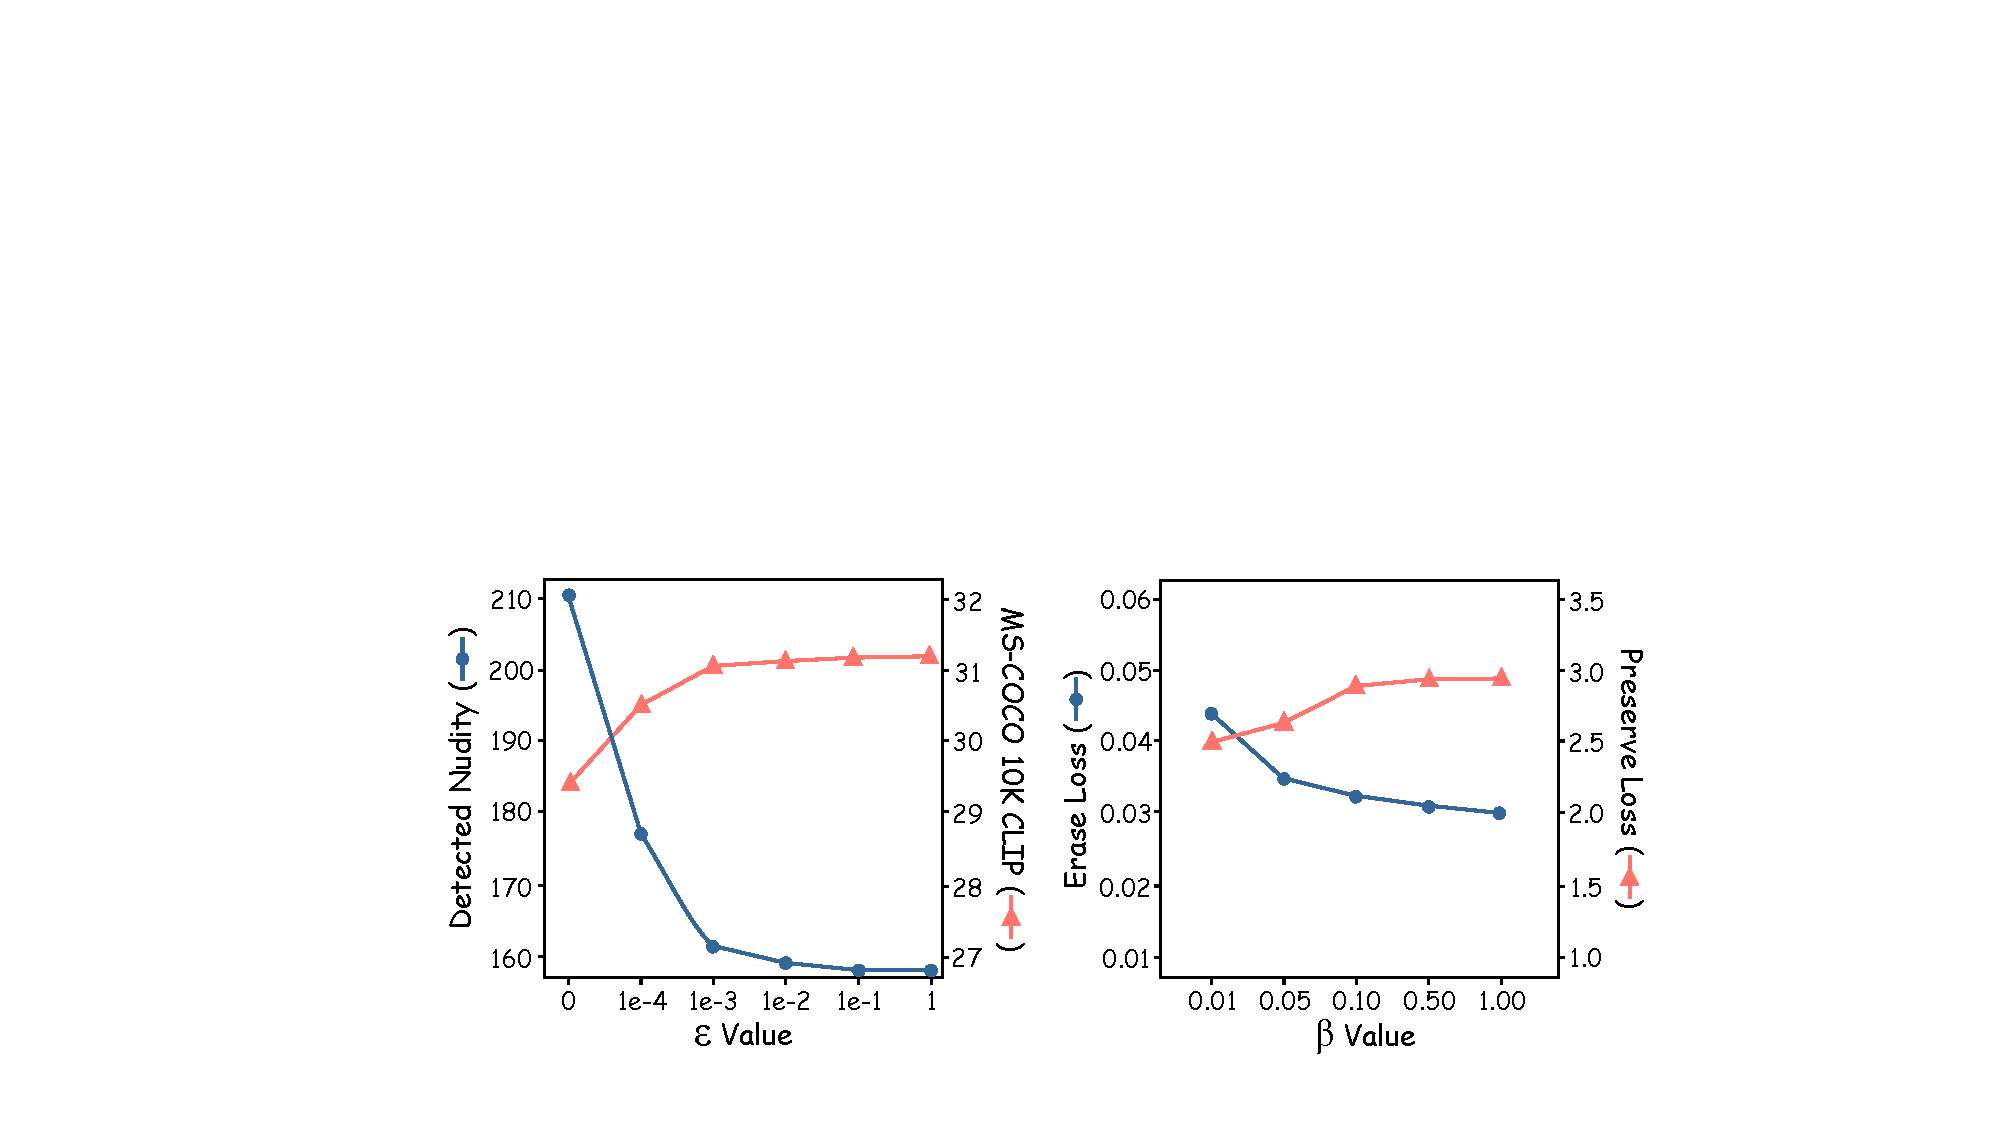
\includegraphics[width=0.9\linewidth]{fig/ablation_study_hyber.pdf}
    \caption{\textbf{Ablation study on hyperparameters $\varepsilon$ and $\beta$}. With our \emph{Lagrangian-Guided Adaptive Erasure Modulation} algorithm, erasure and preservation become monotonically controllable.}
    \label{fig:ablation_study_hyber}
    \vspace{-5pt}
\end{figure}


\textbf{Ablation on Stream Disentangled Concept Erasure Framework.}
We first validate the structural necessity of our framework. As visualized in Appendix Fig.~\ref{fig:ablation_nude}, naive fine-tuning on single-stream models consistently causes generation collapse regardless of layer selection, proving our framework is a prerequisite for stable erasure. Within this safe subspace, we further ablate our loss terms in \cref{tab: ablation study}. $\mathcal{L}_{erase}$ effectively removes concepts but degrades quality, while $\mathcal{L}_{attn}$ enhances erasure precision. Crucially, $\mathcal{L}_{pr}$ serves as a stabilizer for visual utility. Combining all three yields the optimal equilibrium between safety and quality.




\textbf{Ablation on Lagrangian-Guided Adaptive Erasure Modulation.}
We then examine the optimization dynamics by varying tolerance $\varepsilon$ and learning rate $\beta$ in Fig.~\ref{fig:ablation_study_hyber}. 
Consistent with Section~\ref{section: Constraint-Aware Dynamic Balancing}, a smaller $\varepsilon$ favors preservation at the cost of weaker erasure. We thus select $\varepsilon = 0.001$ for balance. In contrast, our method shows strong robustness to $\beta$ with negligible performance fluctuations, verifying that convergence is stable to step size. We set $\beta=0.1$ as a practical choice.
